\documentclass[../discrete.tex]{subfiles}
\graphicspath{{\subfix{../figures/}}}
\begin{document}
\chapter{Counting}
\section{The Basics of Counting}
\begin{definition}
    The Product Rule: Suppose that a procedure can be broken down into a sequence
    of two tasks. If there are $n_1$ ways to do the first task and for each of these ways of doing the 
    first task, there are $n_2$ ways to do the second task, then there are $n_1n_2$ ways to do the procedure.
\end{definition}

\begin{definition}
    The Sum Rule: If a task can be done either in one of $n_1$ ways or in one of $n_2$
    ways, where none of the set of $n_1$ ways is the same as any of the set of $n_2$ ways, then there are 
    $n_1+n_2$ ways to do the task.
\end{definition}

\begin{definition}
    The Subtraction Rule: If a task can be done in either $n_1$ ways or $n_2$ ways, 
    then the number of ways to do the task if $n_1+n_2$ minus the number of ways to do the task 
    that are common to the two different ways.
\end{definition}

\begin{definition}
    The Division Rule: There are $n/d$ ways to do a task if it can be done using a procedure 
    that can be carried out in $n$ ways, and for every way $w$, exactly $d$ of the $n$ ways 
    correspond to way $w$.
\end{definition}
\section{The Pigeonhole Principle}
\begin{theorem}
    The Pigeonhole Principle: If $k$ is a positive integer and $k+1$ or more 
    objects are placed into $k$ boxes, then there is at least one box containing two or more of the objects.
\end{theorem}

\begin{corollary}
    A function $f$ from a set with $k+1$ or more elements to a set with $k$ elements is not one-to-one.
\end{corollary}

\begin{theorem}
    The Generalized Pigeonhole Principle: If $N$ objects are placed into $k$ boxes, then 
    there is at least one box containing at least $\lceil N/k \rceil$ objects.
\end{theorem}

\begin{theorem}
    Every sequence of $n^2+1$ distinct real numbers contains a subsequence of length $n+1$ that is either strictly increasing or strictly decreasing.
\end{theorem}
\section{Permuations and Combinations}
\begin{theorem}
    If $n$ is a positive integer and $r$ is an integer with $1\leq r\leq n$, then there are 
    \[P(n,r)=n(n-1)(n-2)\cdots(n-r+1)\]
    $r$-permutations of a set with $n$ distinct elements.
\end{theorem}

\begin{corollary}
    If $n$ and $r$ are integers with $0\leq r\leq n$, then $P(n,r)=\frac{n!}{(n-r)!}$.
\end{corollary}

\begin{theorem}
    The number of $r$-combinations of a set with $n$ elements, where $n$ is a nonnegative integer
    and $r$ is an integer with $0\leq r\leq n$, equals 
    \[C(n,r)=\frac{n!}{r!(n-r)!}\]
\end{theorem}

\begin{corollary}
    Let $n$ and $r$ be nonnegative integers with $r\leq n$. Then $C(n,r)=C(n,n-r)$.
\end{corollary}

\begin{definition}
    A combinatorial proof of an identity is a proof that uses counting arguments to prove that 
    both sides of the identity count the same objects but in different ways or a proof that is based 
    on showing that there is a bijection between the sets of objects counted by the two sides of the identity.
    These two types of proofs are called double counting proofs and bijective proofs, respectively.
\end{definition}


\section{Binomial Coefficients and Identities}
The number of $r$-combinations from a set with $n$ elements is often denoted by $\binom{n}{r}$. This number is also called a binomial 
coefficient because these numbers occur as coefficients in the expansion of powers of binomial expressions such as 
$(a+b)^n$.

The binomial theorem gives the coefficients of the expansion of powers of binomial expressions.
A binomial expression is simply the sum of two terms, such as $x+y$.
\begin{theorem}
    Let $x$ and $y$ be variables, and let $n$ be a nonnegative integer. Then 
    \[(x+y)^n=\sum_{j=0}^n\binom{n}{j}x^{n-j}y^j = \binom{n}{0}x^n+\binom{n}{1}x^{n-1}y+\cdots+\binom{n}{n-1}xy^{n-1}+\binom{n}{n}y^n\]
\end{theorem}

We can prove some useful identities from this.
\begin{corollary}
    Let $n$ be a nonnegative integer. Then 
    \[\sum_{k=0}^n\binom{n}{k}=2^n\]
\end{corollary}

\begin{corollary}
    Let $n$ be a positve integer. Then 
    \[\sum_{k=0}^{n}(-k)^k\binom{n}{k}=0\]
\end{corollary}

\begin{corollary}
    Let $n$ be a nonnegative integer. Then 
    \[\sum_{k=0}^n 2^k\binom{n}{k}=3^n\]
\end{corollary}

The binomial coefficients satisfy many different identities. We introduce one of the most important of these now.
\begin{theorem}
    Let $n$ and $k$ be positive integers with $n\geq k$. Then 
    \[\binom{n+1}{k}=\binom{n}{k-1}+\binom{n}{k}\]
\end{theorem}

\begin{theorem}
    Let $m$, $n$, and $r$ be nonnegative integers with $r$ not exceeding either $m$ or $n$. Then 
    \[\binom{m+n}{r}=\sum_{k=0}^r \binom{m}{r-k}\binom{n}{k}\]
\end{theorem}

\begin{corollary}
    If $n$ is a nonnegative integer, then 
    \[\binom{2n}{n}=\sum_{k=0}^n \binom{n}{k}^2\]
\end{corollary}

\begin{theorem}
    Let $n$ and $r$ be nonnegative integers with $r\leq n$. Then 
    \[\binom{n+1}{r+1}=\sum_{j=r}^n\binom{j}{r}\]
\end{theorem}

\section{Generalized Permuations and Combinations}
\pagebreak 

\begin{theorem}
    The number of $r$-permutations of a set of $n$ objects with repetition allowed is $n^r$.
\end{theorem}

\begin{theorem}
    There are $C(n+r-1,r)=C(n+r-1,n-1)$ $r$-combinations from a set with $n$ elements when repetition of elements is allowed.
\end{theorem}

\begin{center}
    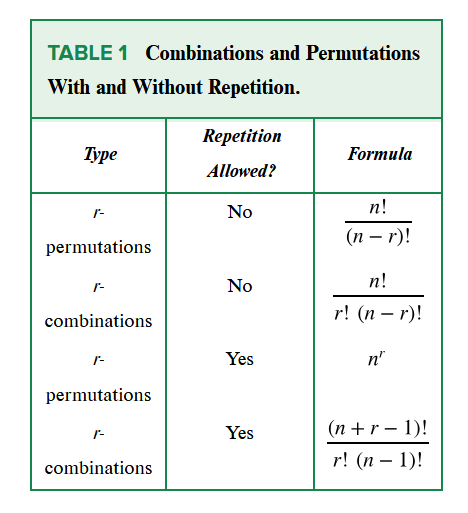
\includegraphics[width=0.6\textwidth]{6.4.PNG}
\end{center}
\begin{theorem}
    The number of different permutations of $n$ objects, where there are $n_1$ indistinguishable objects of type 1, $n_2$ indistinguishable objects of 
    type 2, $\dots$, and $n_k$ indistinguishable objects of type $k$, is 
    \[\frac{n!}{n_1!n_2!\cdots n_k!}\]
\end{theorem}
\begin{theorem}
    The number of ways to distribute $n$ distinguishable objects into $k$ distinguishable boxes so that $n_i$ objects 
    are placed into box $i$, $i=1,2,\dots,k$ equals 
    \[\frac{n!}{n_1!n_2!\cdots n_k!}\]
\end{theorem}

There are $C(n+r-1, n-1)$ ways to place $r$ indistinguishable objects into $n$ distinguishable boxes.


\end{document}